\documentclass[12pt]{article}
\usepackage{graphicx}
\usepackage{amsmath}
\usepackage{mathtools}
\let\vec\mathbf
\begin{document}
\begin{center}
\textbf\large{CHAPTER-7 \\ COORDINATE GEOMETRY}

\end{center}
\section*{Excercise 7.4}

Q4.The two opposite vertices of a square are $(–1, 2) \text{ and } (3, 2)$. Find the coordinates of the other two vertices.\\

\textbf{Solution}: $A =
\begin{pmatrix}
-1 \\
 2
\end{pmatrix},
C = 
\begin{pmatrix}
3\\
2
\end{pmatrix}$

Let $B = \begin{pmatrix}
x\\
y
\end{pmatrix}$

From the properties of square we know that
 $\lVert \vec{AB} \rVert = \lVert \vec{BC} \rVert$\\
 
 $\vec{AB} = \vec{B} - \vec{A} = \begin{pmatrix}
x+1 \\
 y-2
\end{pmatrix} \text{ and }
\vec{BC} = \vec{C} - \vec{B} = \begin{pmatrix}
3-x \\
 2-y
\end{pmatrix}$\\

Now using $\lVert \vec{AB} \rVert = \lVert \vec{BC} \rVert$\\
\begin{align}
\sqrt{(x+1)^{2} + (y-2)^{2}} &= \sqrt{(3-x)^{2} + (2-y)^{2}} \\
(x+1)^{2} &= (3-x)^{2}\\
x^{2}+1+2x &= 9+x^{2}-6x\\
8x &= 8\\
x &= 1
\end{align}\\
Now we also know that two sides of a square are perpendicular to each other.\\
$\vec{AB} \perp \vec{BC}$

\begin{align}
(\vec{AB})^{T}(\vec{BC}) &= 0\\
\begin{pmatrix}
x+1 &
 y-2
 \end{pmatrix}
\begin{pmatrix}
3-x \\
2-y
\end{pmatrix} &= 0\text{ (substituting value of x)}\\
\begin{pmatrix}
2 &
 y-2
 \end{pmatrix}
\begin{pmatrix}
2 \\
2-y
\end{pmatrix} &= 0  \\
4 + (y-2)(2-y) &= 0\\
4 + 2y - y^{2} - 4 + 2y &= 0\\
y^{2} - 4y &= 0\\
y(y - 4) &= 0\\
y &= 0,4
\end{align}

Therefore the other two vertices are $(1,0)\text{ and }(1,4)$

\begin{figure}[!h]
	\begin{center} 
	    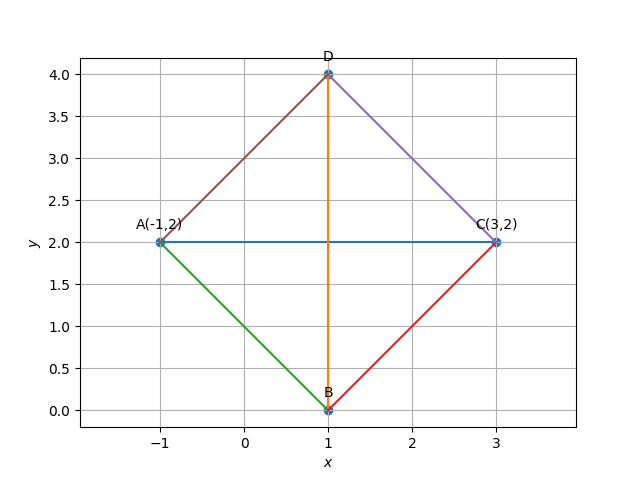
\includegraphics[width=\columnwidth]{./square}
	\end{center}
\caption{}
\label{fig:Fig1}
\end{figure}











\end{document}